\vspace{1em}
\textbf{3.3. Метод на основе неявной разностной схемы.}
\vspace{0.5em}

Этот метод основан на использовании консервативной разностной схемы для неравномерных сеток в поперечном сечении и был предложен в \cite{SweepScheme}.
Она выглядит следующим образом:
\begin{equation}\label{Sweep_Diff_Sys_General_Conservative}
    \left\{
    \begin{aligned}
        2i\frac{h_1}{2}\frac{\hat{E}_{0,j}-E^k_{0,j}}{\Delta z} & = \frac{1}{2}\left(\frac{\hat{E}_{1,j}-\hat{E}_{0,j}}{h_1}\right) + \frac{1}{2}\left(\frac{E^k_{1,j}-E^k_{0,j}}{h_0}\right)\\
        2i\frac{h_{i+1}+h_i}{2}\frac{\hat{E}_{i,j}-E^k_{i,j}}{\Delta z} & = \frac{1}{2}\left(\frac{\hat{E}_{i+1,j}}{h_{i+1}} -\left(\frac{1}{h_{i+1}} + \frac{1}{h_i}\right)\hat{E}_{i,j} + \frac{\hat{E}_{i-1,j}}{h_i}\right) \\
        & \qquad+ \frac{1}{2}\left(\frac{E^k_{i+1,j}}{h_{i+1}} -\left(\frac{1}{h_{i+1}} + \frac{1}{h_i}\right)E^k_{i,j} + \frac{E^k_{i-1,j}}{h_i}\right),\quad i=1,\ldots N\\
        2i\frac{h_N}{2}\frac{\hat{E}_{N,j}-E^k_{N,j}}{\Delta z} & = \frac{1}{2}\left(\frac{\hat{E}_{N,j}-\hat{E}_{N-1,j}}{h_N}\right) + \frac{1}{2}\left(\frac{E^k_{N,j}-E^k_{N,j}}{h_{N-1}}\right)
    \end{aligned}
    \right.
\end{equation}
где  $h_i=x_i-x_{i-1}$.

Указанная схема осуществляет расчёт <<дифракции по $x$>>. Аналогичная система разностных уравнений рассчитывает <<дифракцию по $y$>>.
Если шаг сетки равномерный, то есть $h_i=h=const$, то схема переходит в хорошо известную схему Кранка-Николсона:
\begin{equation}\label{Sweep_Diff_Sys_Crank_Nicholson}
    \left\{
    \begin{aligned}
        2i\frac{\hat{E}_{0,j}-E^k_{0,j}}{\Delta z} & = \left(\frac{\hat{E}_{1,j}-\hat{E}_{0,j}}{h^2}\right) + \left(\frac{E^k_{1,j}-E^k_{0,j}}{h^2}\right)\\
        2i\frac{\hat{E}_{i,j}-E^k_{i,j}}{\Delta z} & = \frac{1}{2}\left(\frac{\hat{E}_{i+1,j} - 2\hat{E}_{i,j} + \hat{E}_{i-1,j}}{h^2}\right) \\
                                                    & + \frac{1}{2}\left(\frac{E^k_{i+1,j} - 2E^k_{i,j} + E^k_{i-1,j}}{h^2}\right), \quad i = 1, \ldots, N\\
        2i\frac{\hat{E}_{N,j}-E^k_{N,j}}{\Delta z} & = \left(\frac{\hat{E}_{N,j}-\hat{E}_{N-1,j}}{h^2}\right) + \left(\frac{E^k_{N,j}-E^k_{N,j}}{h^2}\right)
    \end{aligned}
    \right.
\end{equation}

Указанная система является системой относительно значений поля на промежуточном слое~$\hat{E}_{i,j}$.
Матрицы систем (\ref{Sweep_Diff_Sys_General_Conservative}) и (\ref{Sweep_Diff_Sys_Crank_Nicholson}) трехдиагональная, а значит их можно решать методом прогонки \cite{Kalitkin}.
Рассмотрим параллельную реализацию метода прогонки.

\begin{figure}[h]
    \begin{center}
        \begin{minipage}{0.45\linewidth}
            \center{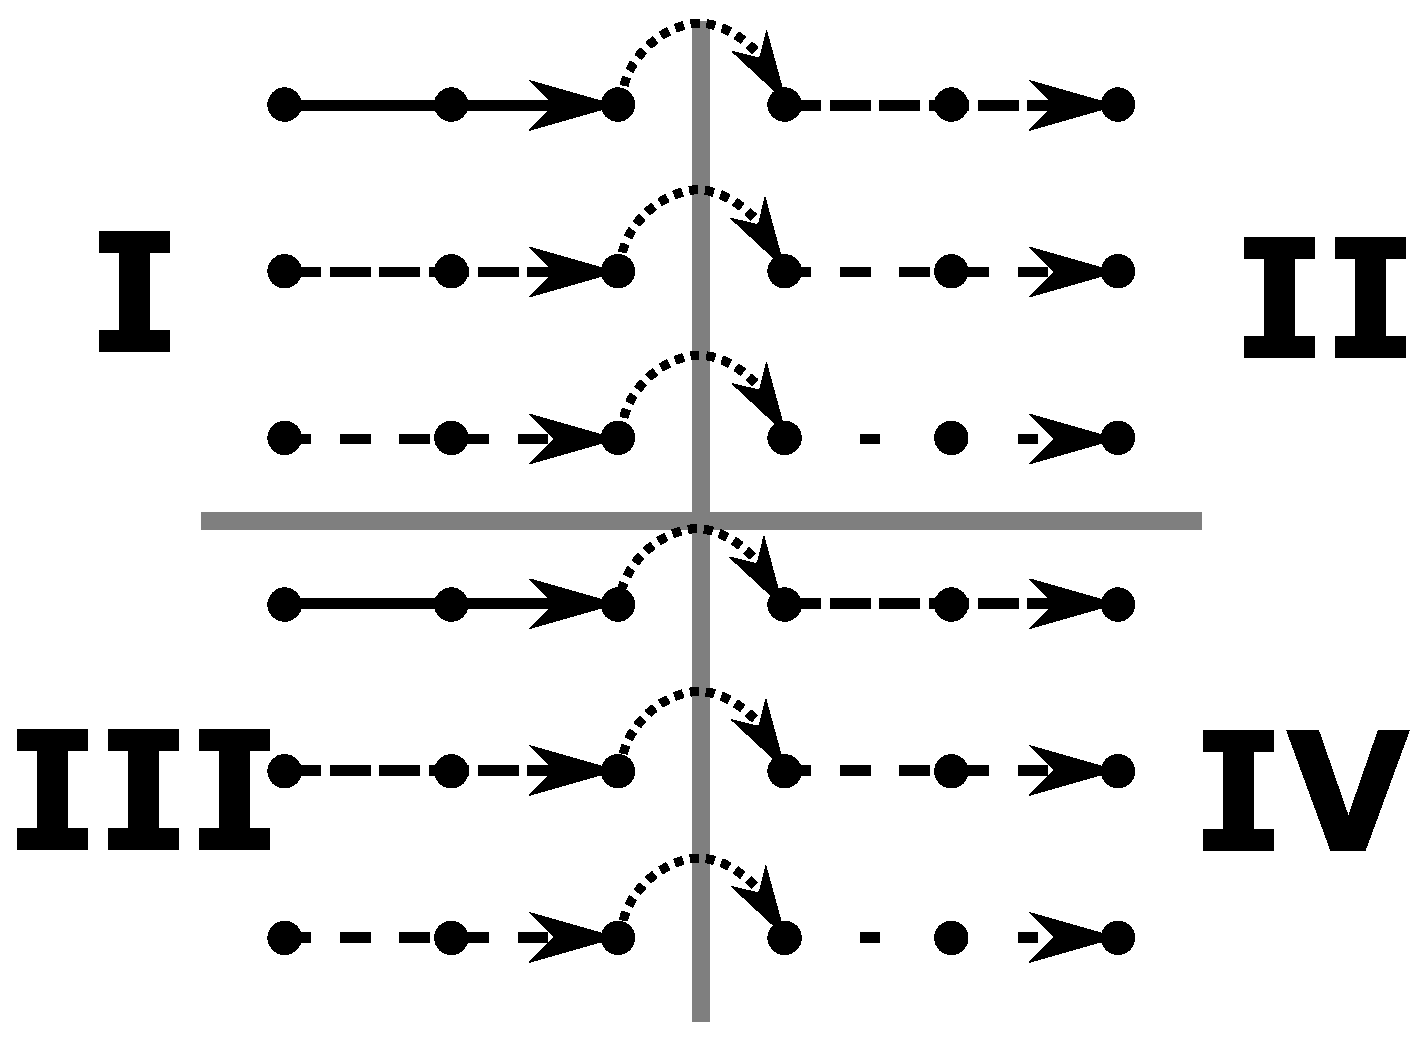
\includegraphics[width=0.95\linewidth]{\imagesdir/sweep_method_forward}} \\
            \caption{Прямая прогонка.}
            \label{img:sweepforward}
        \end{minipage}
        \hfill
        \begin{minipage}{0.45\linewidth}
            \center{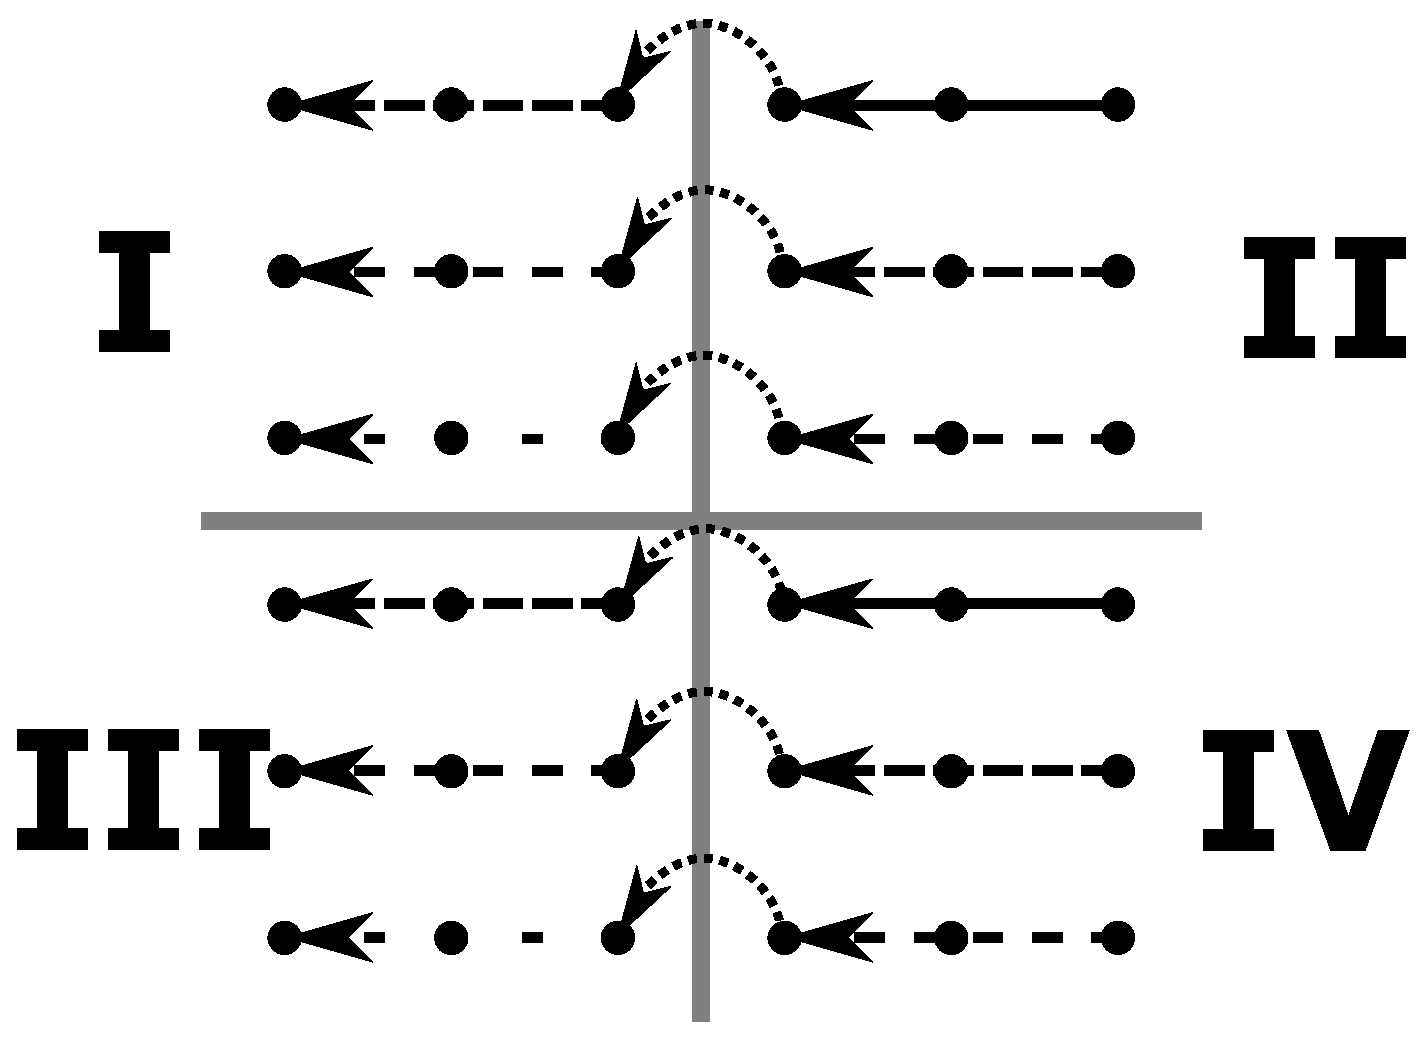
\includegraphics[width=0.95\linewidth]{\imagesdir/sweep_method_backward}} \\
            \caption{Обратная прогонка.}
            \label{img:sweepbackward}
        \end{minipage}
    \end{center}
\end{figure}

На рис. \ref{img:sweepforward}, \ref{img:sweepbackward} черными точками изображены точки расчетной сетки.
Вертикальная и горизонтальная светло-серые прямые показывают разбиение матрицы поперечного сечения между процессами.
Римские цифры обозначают номера процессов.
Стрелки соответствуют вычислению прогоночных коэффициентов.
Стрелки точками отображают обмены данными между процессами.

Первому расчётному шагу соответствуют сплошная стрелка, а следующим стрелки пунктиром с увеличивающимся расстоянием между штрихами.
Для цикла прямой прогонки их выполняют процессы первого столбца матрицы процессов.
Далее эти процессы пересылают посчитанные коэффициенты в граничной точке соседнему справа процессу.
Таким образом, по каждой строке матрицы процессов запускается конвейерная схема параллельных вычислений.

В цикле обратной прогонки конвейерная схема запускается в обратную сторону (соответствие цвета стрелок и порядка выполнения расчётных операций то же).
Пересылке теперь подвергаются рассчитанные значения поля на промежуточном шаге.

Отметим несколько особенностей данного метода.
Во-первых, поскольку цикл обратной прогонки запускается после окончания прямой прогонки по всем строкам расчётной сетки, то необходимо хранить в памяти прогоночные коэффициенты для всех строк, то есть необходима дополнительная матрица для прогоночных коэффициентов того же размера, что и матрица поля.
Во-вторых, для расчёта коэффициентов, фигурирующих в разностных системах (\ref{Sweep_Diff_Sys_General_Conservative}) и (\ref{Sweep_Diff_Sys_Crank_Nicholson}), необходим обмен значениями поля в граничных областях.
В-третьих, для высокой эффективности параллельного алгоритма необходимо, чтобы количество строк матрицы поля у отдельного процесса было существенно больше количества процессов в строке матрицы процессов.
Действительно, если число строк у отдельного процесса равно $N_{loc}$, а число процессов в строке матрицы процессов равно $q$
(на рис. \ref{img:sweepforward}, \ref{img:sweepbackward} $N_{loc}=3$, $q=2$), то на цикл прямой прогонки потребуется $N_{loc}+q$ итераций.
Таким образом, верхняя оценка на эффективность имеет вид:
\begin{equation}
    E_n\leqslant\frac{N_{loc}q^2}{q^2(N_{loc} + q)}=\frac{1}{1+q/N_{loc}}.
\end{equation}

Заметим, что в этом соотношении не учтены потери времени на пересылки и синхронизацию процессов.

Учёт нелинейности при использовании данного метода осуществляется в рамках описанного в разделе 3. расщепления по физическим факторам.
